\documentclass{article}
\usepackage[german]{babel}
\usepackage[utf8]{inputenc}
\usepackage[a4paper,top=2cm,bottom=2cm,left=3cm,right=3cm,marginparwidth=1.75cm]{geometry}
\usepackage{amsmath}
\usepackage[onehalfspacing]{setspace}
\usepackage{graphicx}
    \graphicspath{ {./images/} }
\usepackage{url}
\usepackage{float}
\usepackage{pdfpages}
\usepackage{lastpage}
\usepackage{siunitx}
\sisetup{separate-uncertainty=true}
\usepackage{gensymb}
\usepackage{indentfirst}
\usepackage[square,numbers]{natbib}
\usepackage[colorlinks=true, allcolors=blue]{hyperref}
\usepackage[headsepline]{scrlayer-scrpage}
\pagestyle{scrheadings}
\clearpairofpagestyles
\begin{document}
\setcounter{totalnumber}{4}
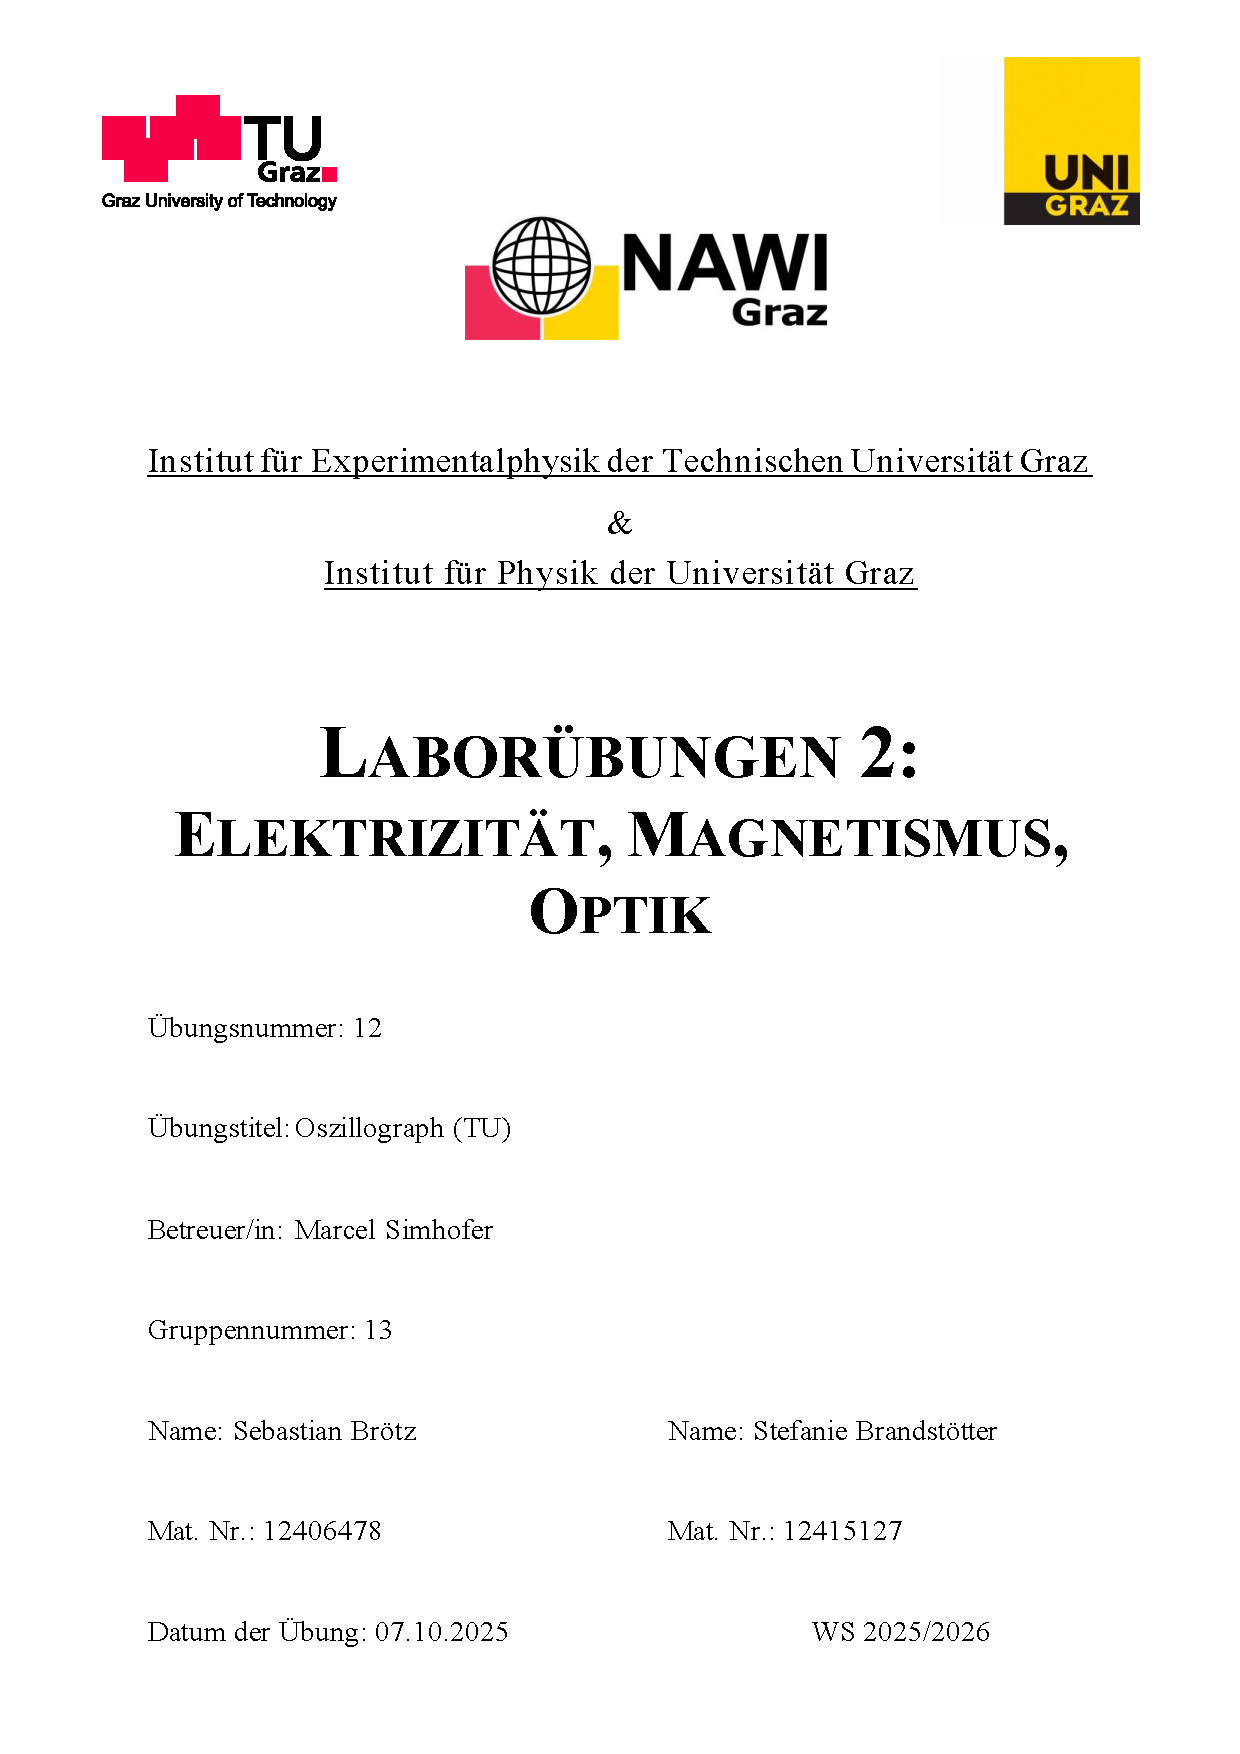
\includepdf{Deckblatt.pdf}

\ihead{Brandstötter, Brötz}
\chead{}
\ohead{}
\cfoot{\thepage{} / \pageref{LastPage}}

\tableofcontents
\newpage

\section{Auswertung}

\begin{figure}[h!]
    \centering
    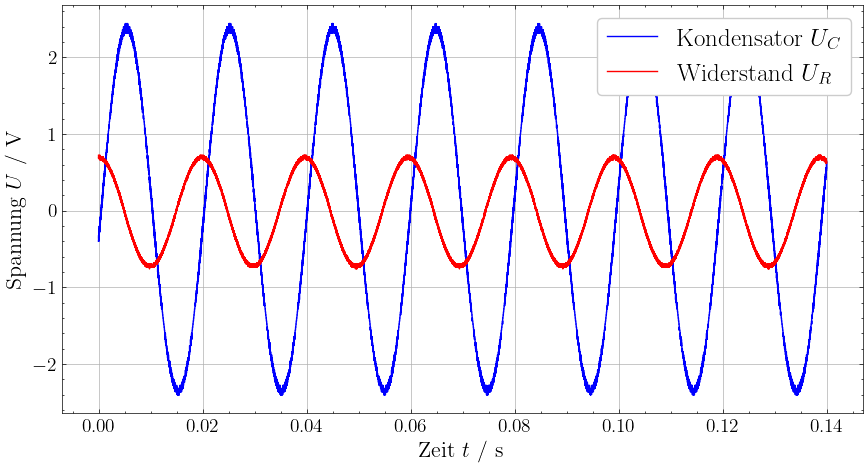
\includegraphics[width=0.8\linewidth]{images/Messung_V1_StromSpannung.png}
    \caption{Aufgezeichnete zeitliche Verläufe der Spannungsabfälle über den Widerstand $R$ und den Kondensator $C$ bei einer sinusförmigen Speisespannung in der Schaltung aus Versuch 1. }
    \label{fig:MessungKondensatorSpannung}
\end{figure}

\begin{table}[h]
    \centering
    \caption{Gemessene Gesamtwiderstände $R_\text{ges}$ inklusive Messunsicherheit dargestellt für die gewählten Potentiometer-Stellungen zur Erzeugung der drei verschiedenen Spannungsverläufe.}
    \label{tab:MessungenWiderstand}
    \begin{tabular}{c|c|c}
         - & \textbf{Widerstand} $R_\text{ges}$ / $\Omega$ & \textbf{Unsicherheit} $\Delta R_\text{ges}$ / $\Omega$ \\\hline
         Kriechfall &  $530$ & $5$ \\ 
         Grenzfall   &  $346$ & $4$ \\
         Schwingfall   &  $85.7$ & $1.0$ \\\hline
    \end{tabular}
\end{table}

\section{Diskussion}
\bibliographystyle{abbrvnat}
\bibliography{lit.bib}
\newpage
\listoffigures
\listoftables
\end{document}